	\begin{figure}[h]
	\centering
		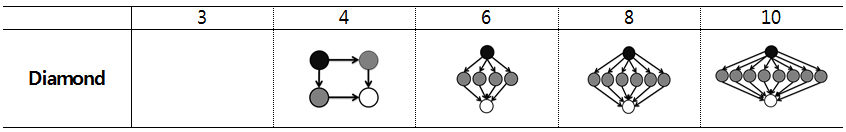
\includegraphics[height=50pt]{images/Topologies_Diamond}
		\caption{Bayesian Network Topologies : Diamond}
	\end{figure}	

	% Diamond는 윗 부분은 한 개의 node가 여러 개의 자식 node를 가진 Star 형태이고, 아래 부분은 한 개의 자식 node가 여러 개의 부모 node를 가진 Collapse 형태이다.
	A part of the top, one node has plurality of child node like Star form. And the bottom part, one node has plurality of parent node like Collapse form. If it connected, then it called Diamond.
	
\begin{figure}[!bhp]
	\centering
		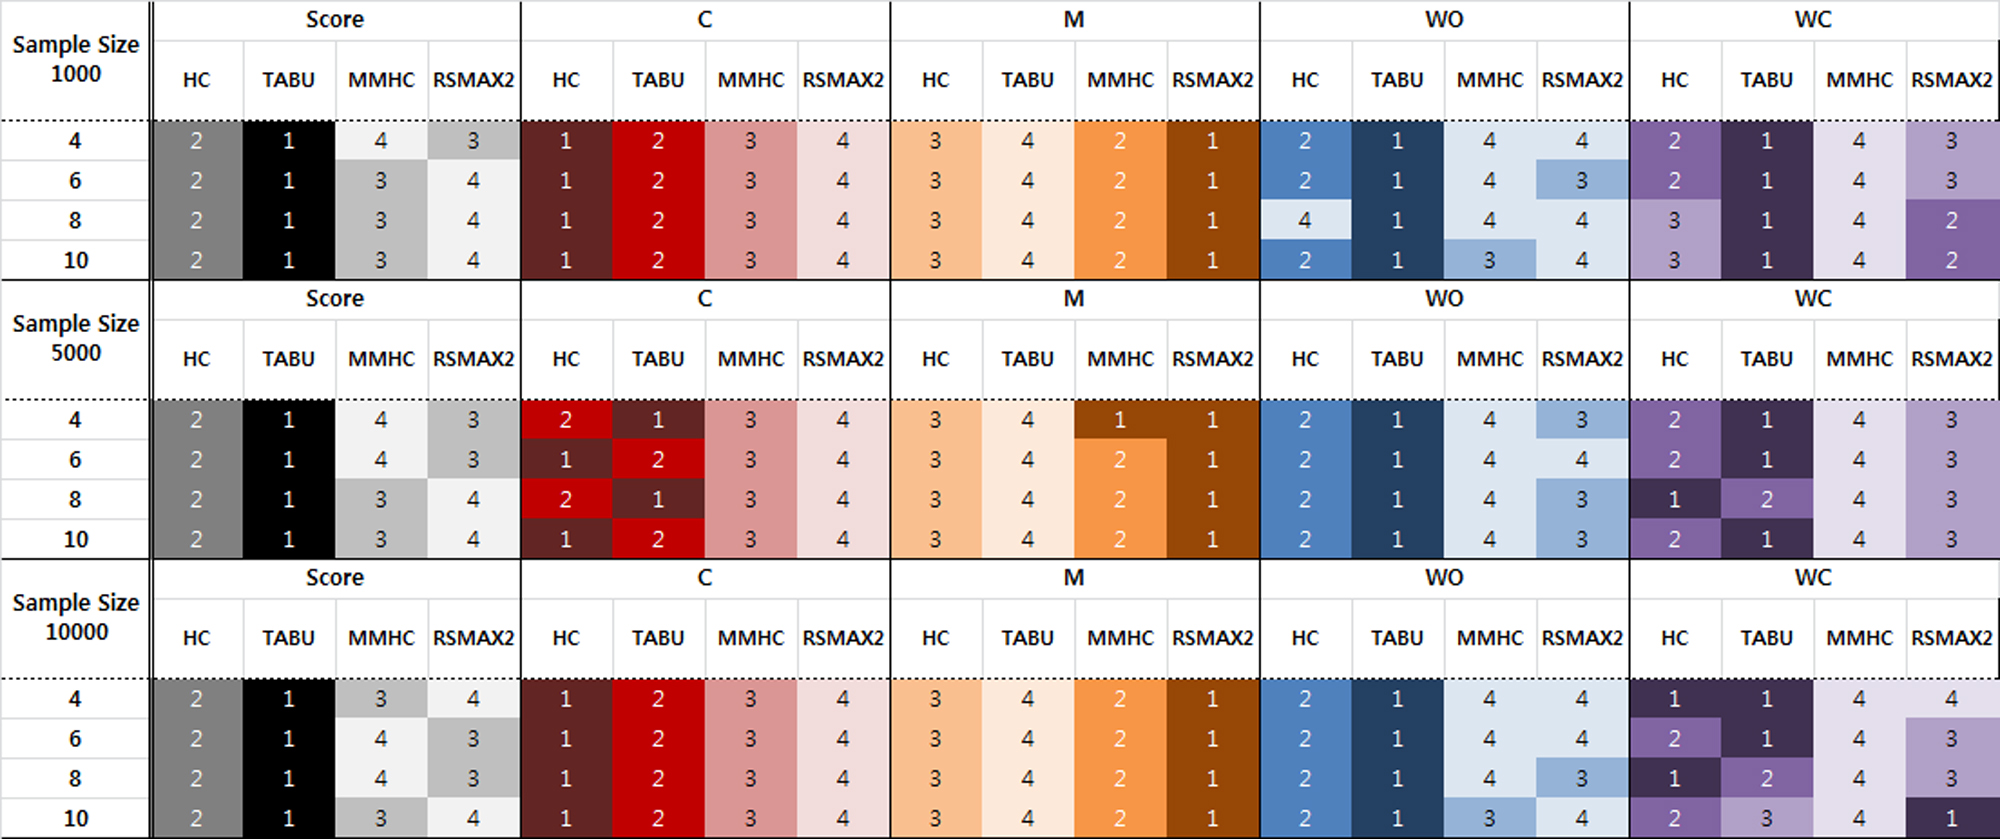
\includegraphics[height=155pt]{images/Result_Diamond}
		\caption{Summary for Comparison via Diamond}
	\end{figure}	

% Score, C 기준으로 비교했을 때 각각 TABU search, Hill-climbing이 좋은 성능을 나타냈다. 하지만 WO, WC도 많은 것으로 나타났다
Respectively, when compared to the score and C,  TABU search and Hill-climbing showed a good performance. However, WO, WC also showed that many.

% WO, WC가 적은 것을 기준으로 보았을 때 MMHC가 유리한 것으로 나타났다. RSMAX2는 WC가 많이 나타났다.
when compared to the WO and WC, MMHC showed that advantageous. RSMAX2 showed a lot of WC.

% 이러한 현상은 sample size가 커질수록, node 개수가 많아질수록 두드러졌다.
This phenomenon was stood out when the larger the sample size or the node.
	
	\begin{figure}[p]
	\centering
		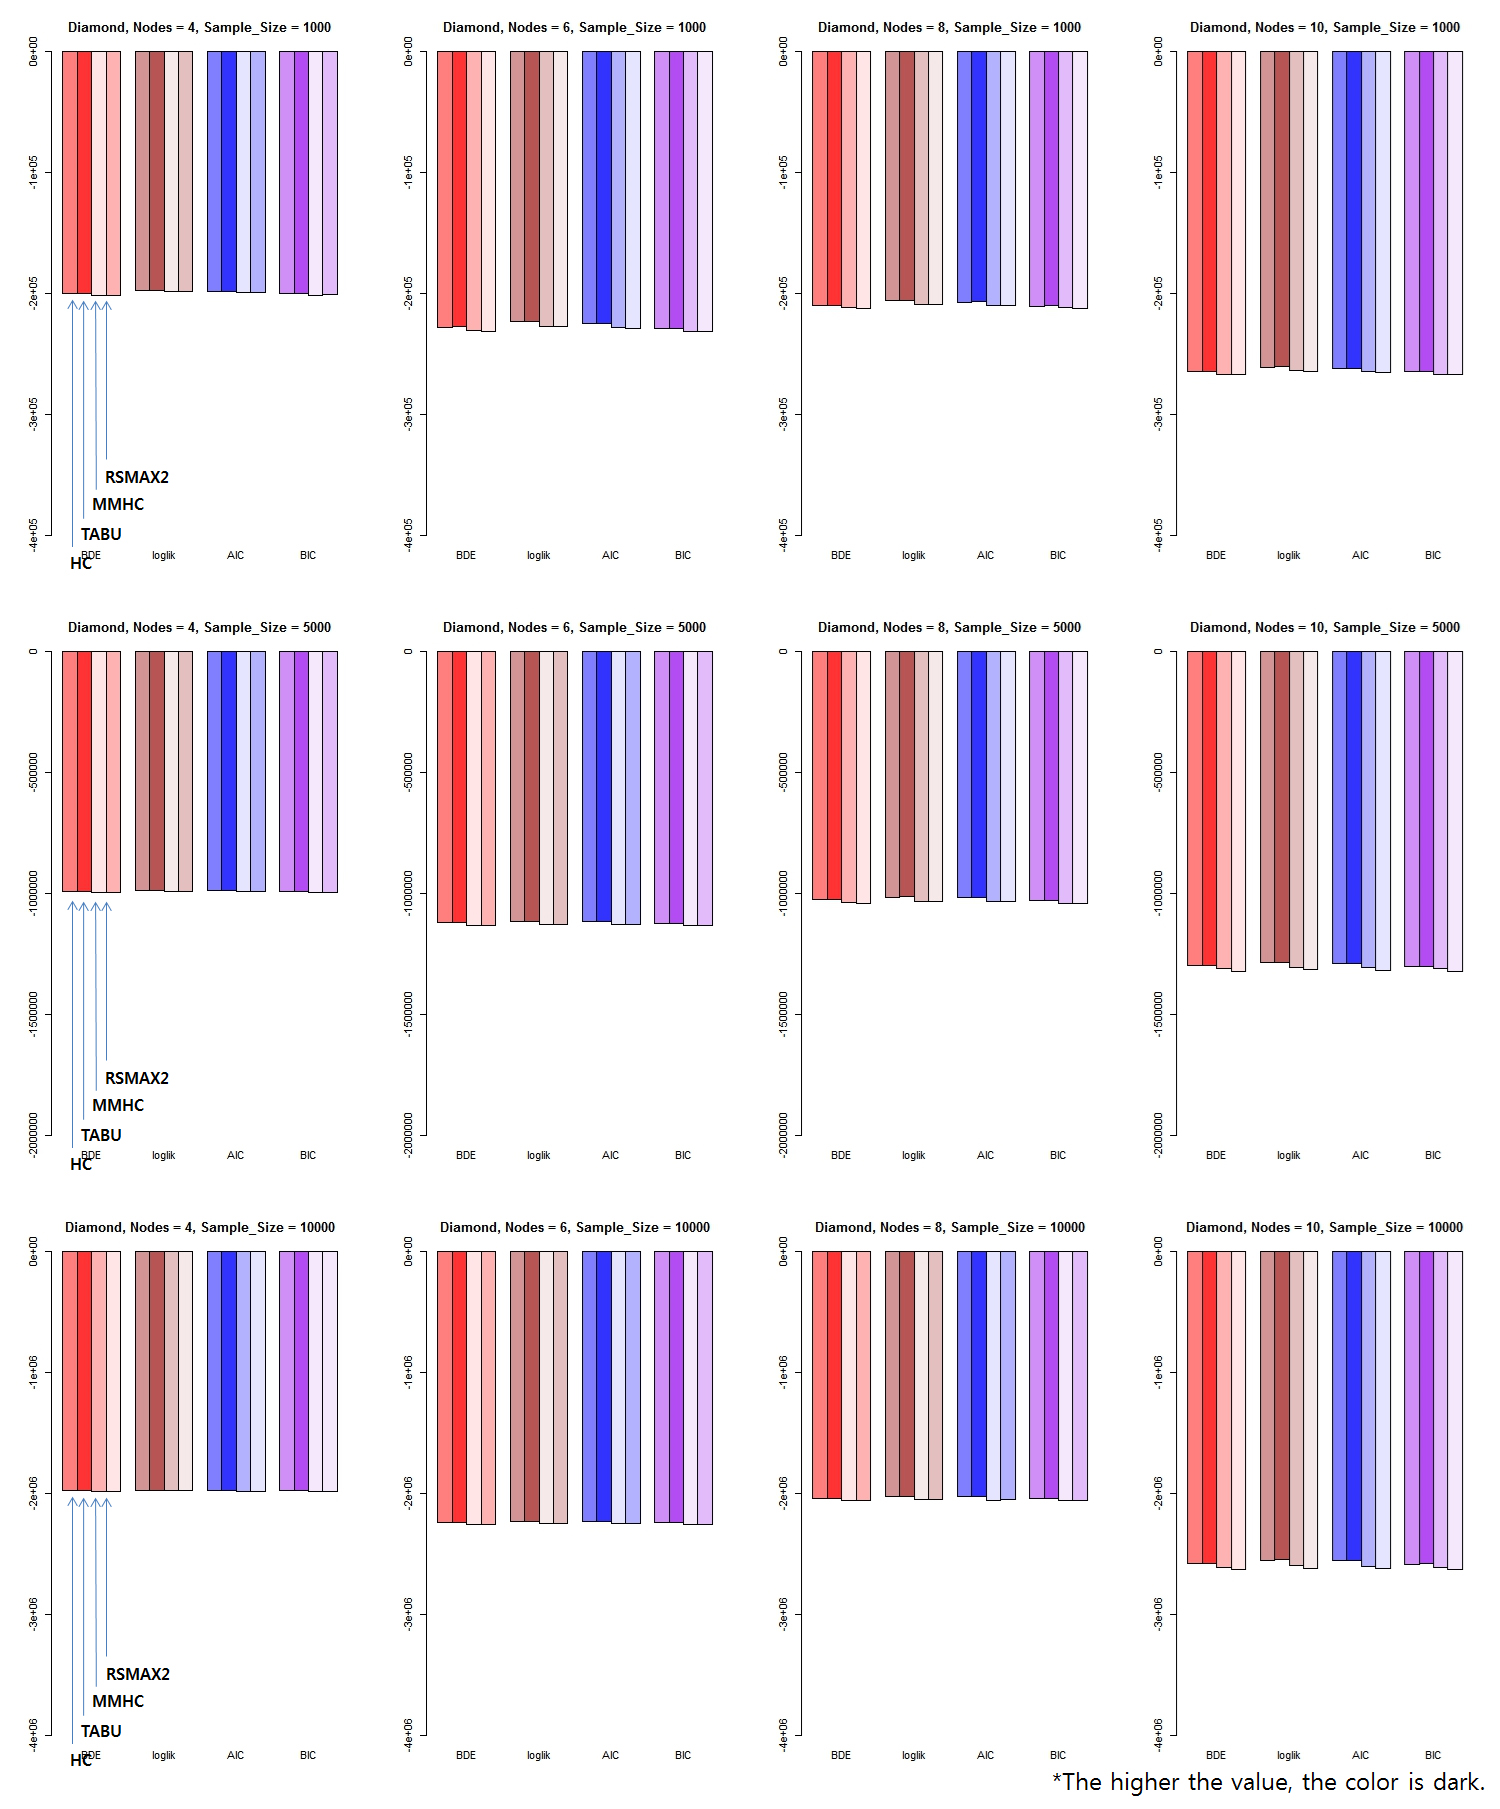
\includegraphics[height=500pt]{images/05_Diamond_Score}
		\caption{Comparison of scores via Diamond}
	\end{figure}	

	\begin{figure}[p]
	\centering
		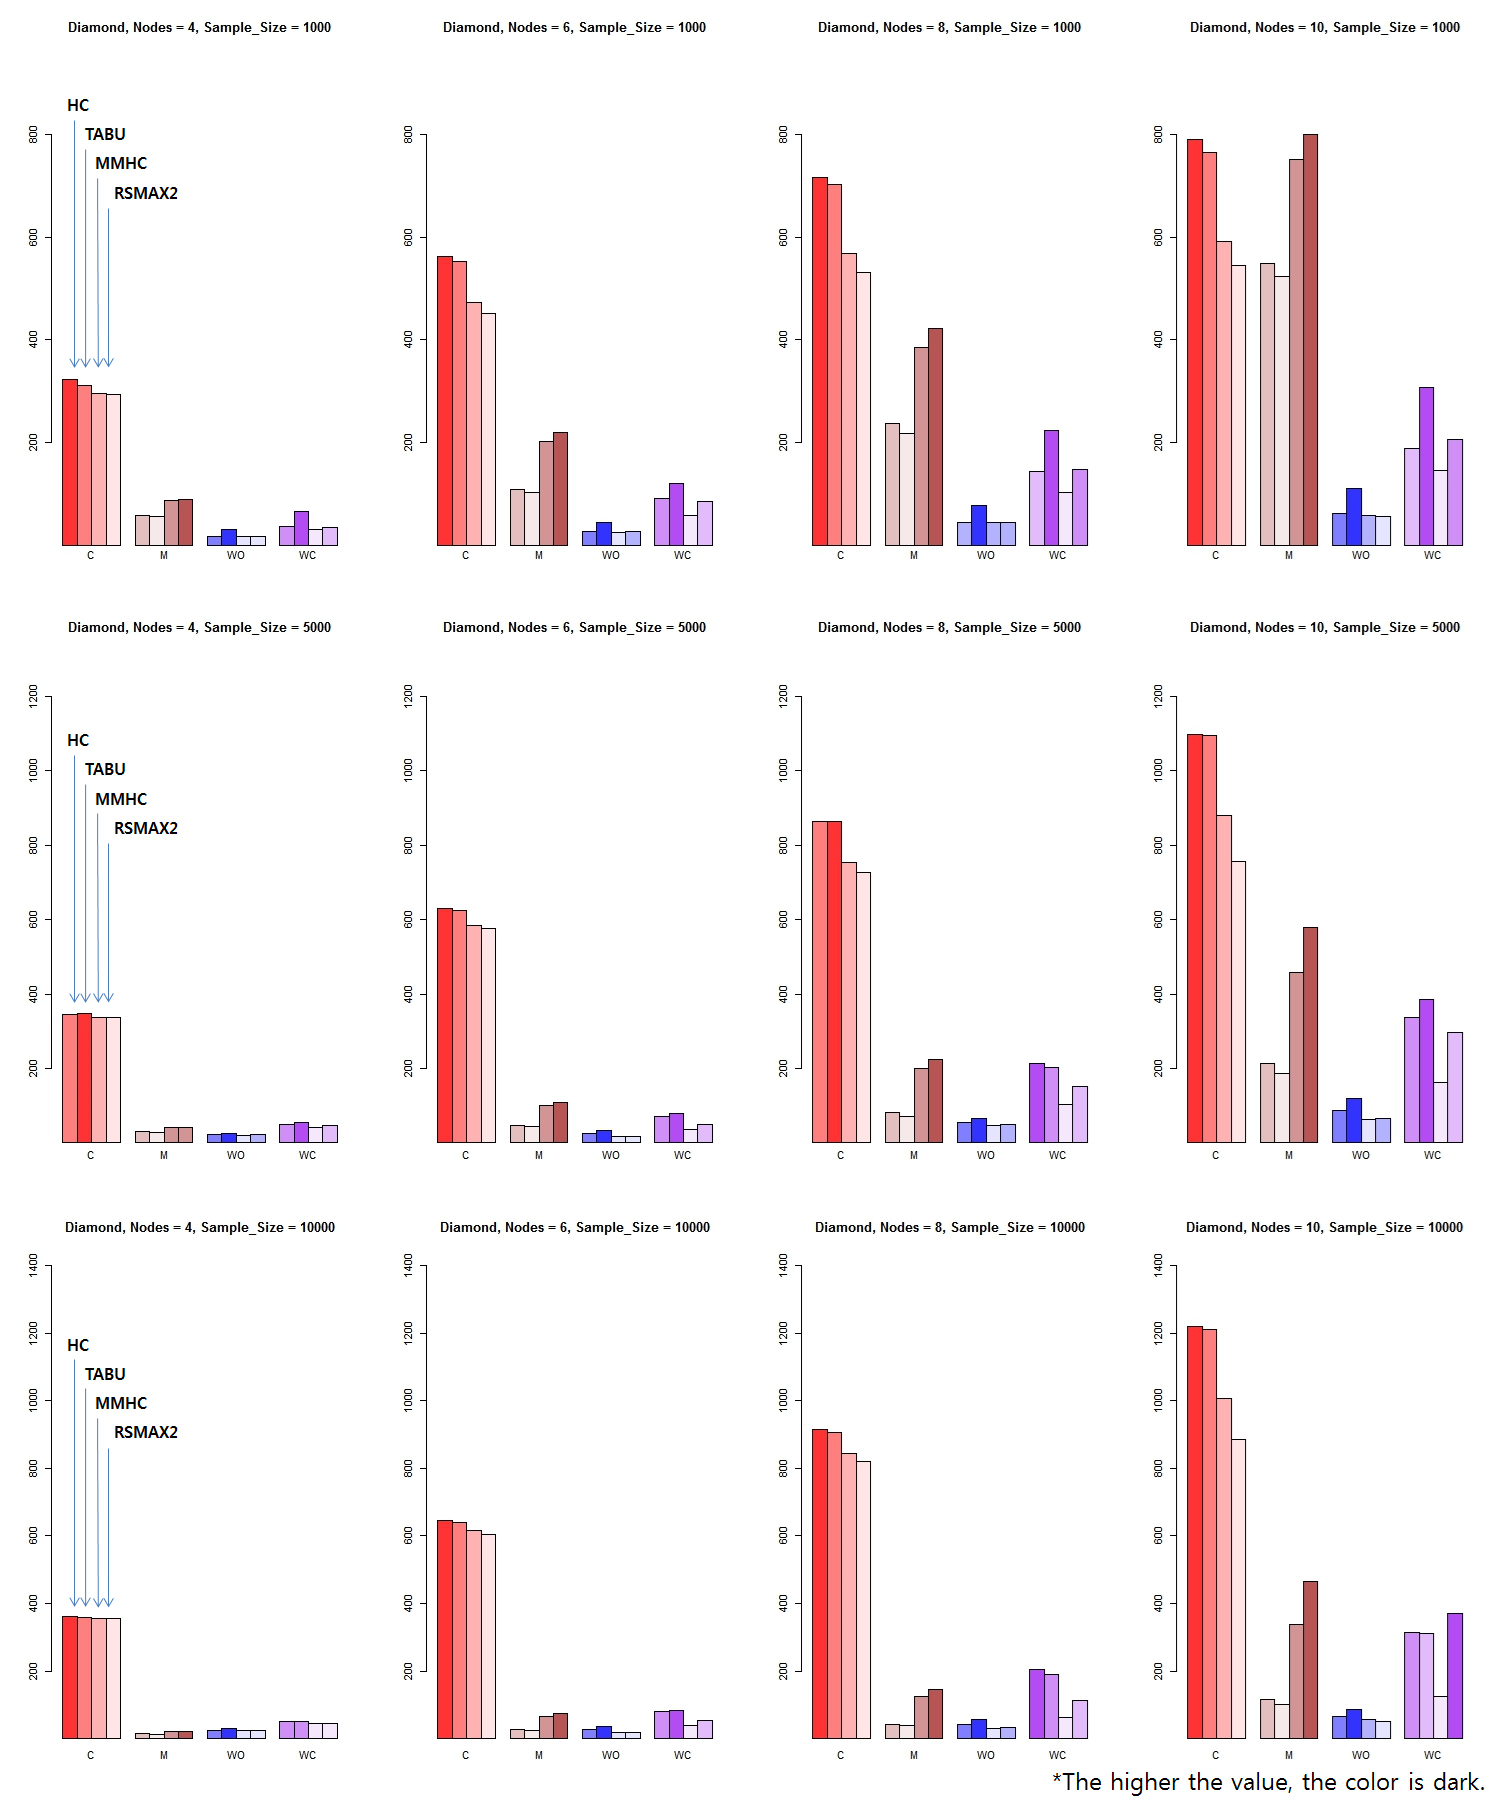
\includegraphics[height=500pt]{images/05_Diamond_Arcs}
		\caption{Comparison of correct arcs via Diamond}
	\end{figure}	
	